\section{Tuning of Tabu}

This section is used to identify and then tune the possible parameters that can alter the results of the Tabu Search algorithm.



The first parameter we tested is the \textit{Tenure Ratio}, a value that in our implementation serves the role of choosing the right \textit{Tenure} (or $T_{max}$) depending on the size of the input instance.

In Figure \ref{fig:tabu} we can see that a \textit{Tenure Ratio} of 2 has to be chosen to obtain the best performance on all the instances used.



The secondo parameter to be tested is the \textit{Tenure} itself. As an initial hypothesis we thought that having a bigger \textit{Tenure}, in the sense of forbidding certain moves for more time, could end up in finding better solutions, but Figure \ref{fig:tabu2} actually shows the opposite.


\begin{figure}[!h]
    \centering
        %Prima riga
        \begin{subfigure}{0.48\textwidth} %Controllo della posizione in orizzontale
            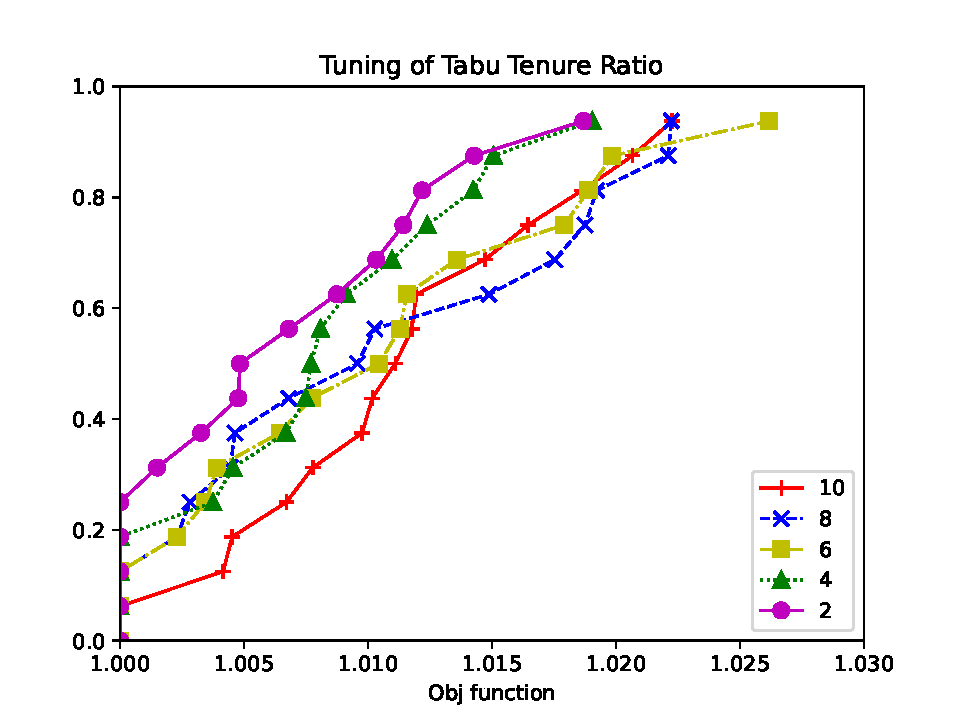
\includegraphics[scale=0.45]{images/tabu.pdf} 
            \caption{Tuning of Tabu Tenure Ratio}
            \label{fig:tabu}
        \end{subfigure}
        \begin{subfigure}{0.48\textwidth}
            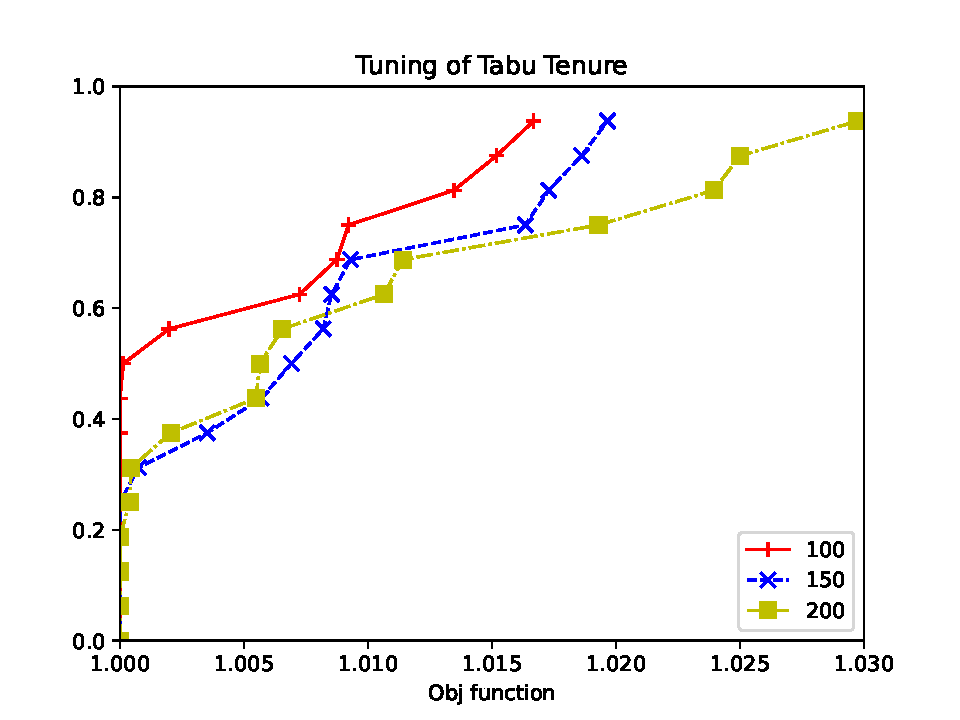
\includegraphics[scale=0.45]{images/tabu2.pdf}
            \caption{Tuning of Tabu Tenure}
            \label{fig:tabu2}
        \end{subfigure}
    \caption{Tuning of Tabu Search}
    \end{figure}